\documentclass[useAMS,usenatbib]{mn2e}
%\documentclass[twocolumn]{emulateapj}
\usepackage{graphicx,natbib,color,multirow,amsmath,url,soul}
\usepackage{epsfig}
\usepackage{float}
\usepackage{deluxetable}

\newcommand\ion[2]{[#1$\;${\scshape{#2}}]}      % ion, i.e., [CII] = \ion{C}{ii}
\newcommand\pfeatures{$p_{\rm{features~or~disk}}$}
\newcommand\plusminus[2]{\genfrac{}{}{0pt}{}{#1}{#2}}
\newcommand\pnotedgeon{$p_{\rm{not~edge-on}}$}
\newcommand\pbar{$p_{\rm{bar}}$}
\newcommand\pnobar{$p_{\rm{no~bar}}$}
\newcommand\gztwo{Galaxy~Zoo~2}
\newcommand\mbh{$M_{\rm{BH}}$}
\newcommand\db{$d_{\rm{B-NB}}$}
\newcommand\fb{$f_{\rm{B>NB}}$}
\newcommand\pasa{PASA}
\voffset-1.25cm
\begin{document}

\title[Galaxy~Zoo: passive disk fraction]{Galaxy~Zoo~Hubble: the passive disk fraction decreases from $z=1.0$ to $z=0.3$ or maybe increases who even knows}
\author[Galloway et~al.]{\parbox[t]{16cm}{Melanie A. Galloway$^1$,several others
\vspace{0.1in} }\\
$^{1}$School of Physics and Astronomy, University of Minnesota, 116 Church St. SE, Minneapolis, MN 55455, USA\\
%$^{2}$Wheelock College, Department of Science, Wheelock College, Boston, MA 02215, USA\\
%$^{3}$Institute for Astronomy, Department of Physics, ETH Z\"urich, Wolfgang-Pauli-Strasse 16, CH-8093, Z\"urich, Switzerland\\
%$^{4}$Department of Astronomy and Astrophysics, 1156 High Street, University of California, Santa Cruz, CA 95064, USA\\
%$^{5}$Kavli IPMU (WPI), The University of Tokyo, Kashiwa, Chiba 277-8583, Japan\\
%$^{6}$Oxford Astrophysics, Denys Wilkinson Building, Keble Road, Oxford OX1 3RH, UK\\
%$^{7}$Institute of Cosmology \& Gravitation, University of Portsmouth, Dennis Sciama Building, Portsmouth PO1 3FX, UK\\
%$^{8}$SEPnet --- \url{http://www.sepnet.ac.uk} \\
   }
\maketitle

\begin{abstract}


\end{abstract}

\section{Introduction}
\label{sec:Intro}

\begin{itemize}
\item main idea: spiral/disk galaxies tend to show ongoing star formation, elliptical/spheroidal galaxies tend to exhibit little to no star formation. Relative numbers of populations are not constant over time - blue cloud : red sequence decreases as Universe evolves, suggesting a morphological evolution of galaxies coupled with quenching of star formation.

\item driver of evolution (morphologically and in SFR) is not known; also not known to what degree the morphological and quenching transformations are linked, or which occurs first

\item significant population of red sequence disks could represent major stage in transformation, for some or all galaxies
 
\end{itemize}

\section{Data}
\label{sec:Data}

The parent sample of galaxies in this paper is drawn from the Galaxy Zoo: Hubble (GZH) catalog (cite Willett et al. 2016), which provides morphological classifications for galaxies sourced from the HST Legacy Surveys. From the main catalog we select galaxies with imaging from the Cosmic Evolution Survey (COSMOS, \citet{Scoville2007}) in the redshift range $0<z<1$. From this, we apply a magnitude cut of $M_{r^{+}}<-20.5$ to create a volume-limited sample (see Figure~\ref{fig:volume_lim}). Rest frame NUV-r and r-J colors are taken from the UltraVISTA catalog \citep{McCracken2012,Ilbert2013}.

\subsection{Selecting passive disk galaxies}
We identify a sample of non-clumpy disk galaxies using the morphological classifications provided by GZH. The sample includes subjects which meet the following criteria: $\rm f_{features} > 0.23$ and $\rm f_{clumpy,no} > 0.30$, where $\rm f$ is the debiased vote fraction. We also require at least 20 votes for each question ($\rm N_{smooth~or~features} \ge 20$ and $\rm N_{clumpy} \ge 20$) to reduce uncertainty in the vote fractions. 

% Figure - mag vs. z (needed??? questionable. useful? also questionable. ) 
\begin{figure}
\centering
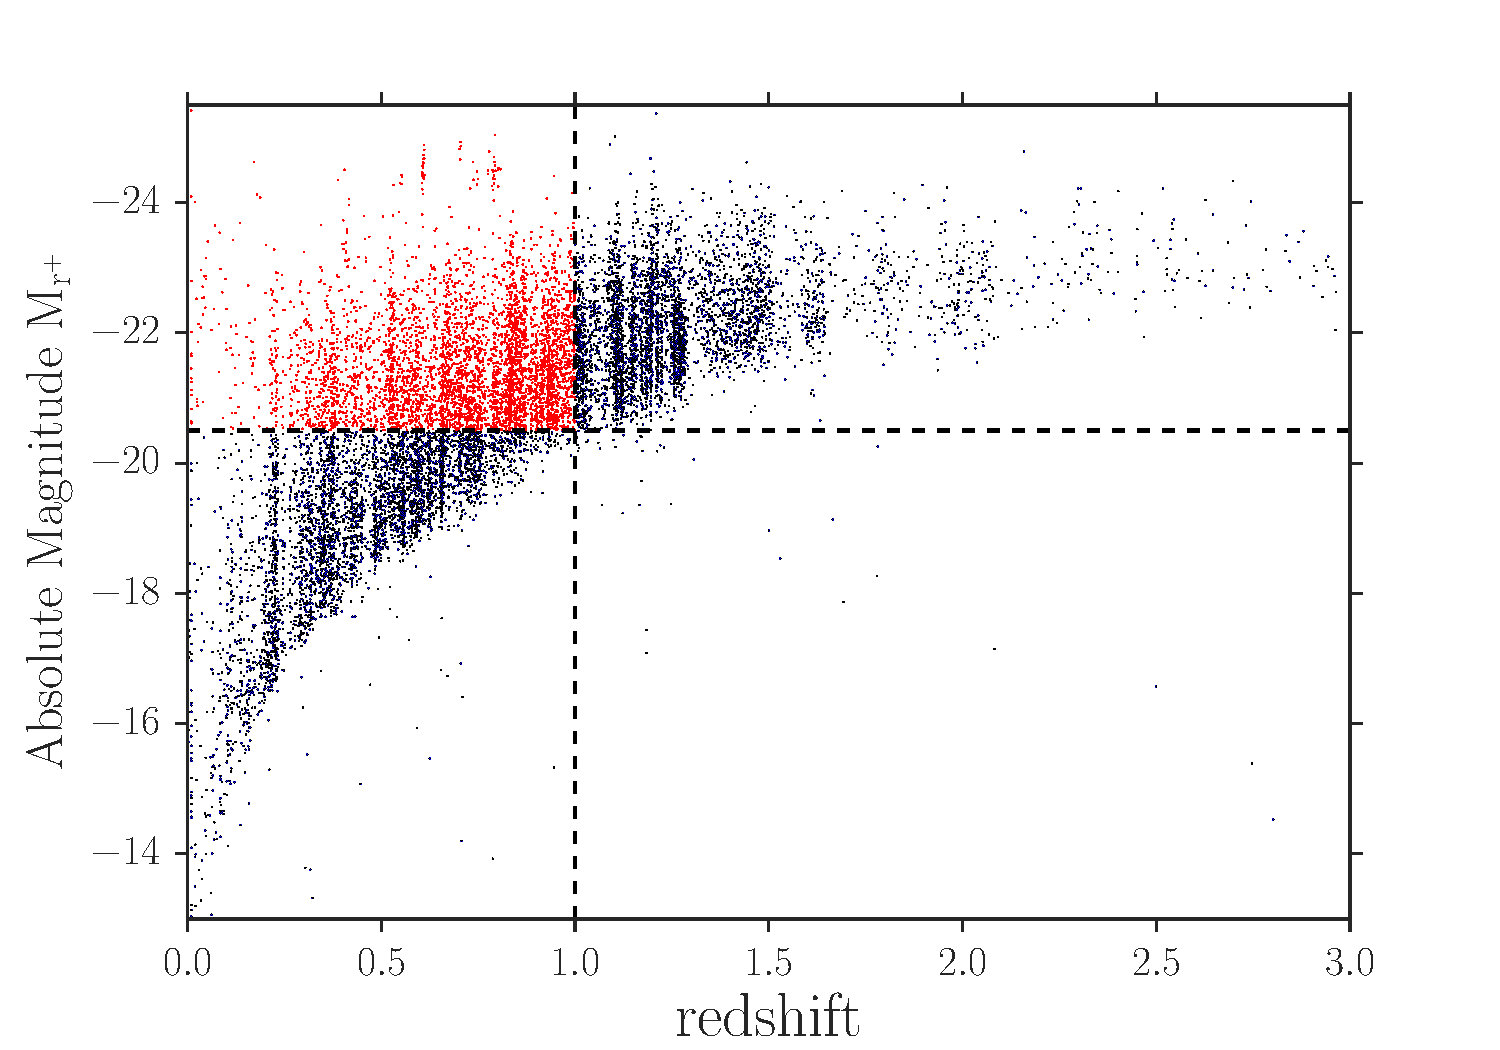
\includegraphics[width=0.45\textwidth]{figures/mag_z_limit.pdf}
\caption{70,198 COSMOS galaxies cross-matched in GZH and UltraVISTA (black). 27,584 are in volume-limited sample (red).}
\label{fig:volume_lim}
\end{figure}   

\section{Ferengi}
\begin{itemize}
\item ~1300ish galaxies, r mags from SDSS \citep{Abazajian2009}
\item NUV mags from GaLEX \citep{Martin2005}
\item J mags from 2Mass \citep{Skrutskie2006}
\end{itemize}
\section{Results}
\label{sec:Results}


\section{Discussion}\label{sec:Discussion}


\section{Conclusions}
\label{sec:conclusions}



%%%%%%%%%%%%
%%% ACKNOWLEDGMENTS
%%%%%%%%%%%%
The data in this paper are the result of the efforts of the Galaxy~Zoo~Hubble volunteers, without whom none of this work would be possible. Their efforts are individually acknowledged at \url{authors.galaxyzoo.org}. Please contact the author(s) to request access to research materials discussed in this paper. 


MG, CS, MB, and LF gratefully acknowledge support from the US National
Science Foundation Grant AST1413610.

This publication makes use of data products from the Two Micron All Sky Survey, which is a joint project of the University of Massachusetts and the Infrared Processing and Analysis Center/California Institute of Technology, funded by the National Aeronautics and Space Administration and the National Science Foundation.

This project made heavy use of the Astropy packages in Python \citep{Robitaille2013}, the \texttt{seaborn} plotting package \citep{Waskom}, and the Tool for OPerations on Catalogues And Tables (TOPCAT), which can be found at \url{www.starlink.ac.uk/topcat/} \citep{topcat2011}. 

Funding for the SDSS and SDSS-II has been provided by the Alfred P. Sloan
Foundation, the Participating Institutions, the National Science Foundation,
the U.S. Department of Energy, the National Aeronautics and Space
Administration, the Japanese Monbukagakusho, the Max Planck Society, and the
Higher Education Funding Council for England. The SDSS website is
\url{http://www.sdss.org/}. 

The SDSS is managed by the Astrophysical Research Consortium for the
Participating Institutions. The Participating Institutions are the American
Museum of Natural History, Astrophysical Institute Potsdam, University of
Basel, University of Cambridge, Case Western Reserve University, University of
Chicago, Drexel University, Fermilab, the Institute for Advanced Study, the
Japan Participation Group, Johns Hopkins University, the Joint Institute for
Nuclear Astrophysics, the Kavli Institute for Particle Astrophysics and
Cosmology, the Korean Scientist Group, the Chinese Academy of Sciences
(LAMOST), Los Alamos National Laboratory, the Max-Planck-Institute for
Astronomy (MPIA), the Max-Planck-Institute for Astrophysics (MPA), New Mexico
State University, Ohio State University, University of Pittsburgh, University
of Portsmouth, Princeton University, the United States Naval Observatory and
the University of Washington. 

\bibliographystyle{mn2e}
\bibliography{/home/mel/Documents/Papers/library}  

\end{document}
